
%(BEGIN_QUESTION)
% Copyright 2006, Tony R. Kuphaldt, released under the Creative Commons Attribution License (v 1.0)
% This means you may do almost anything with this work of mine, so long as you give me proper credit

Hydraulic (liquid) power systems require pressure regulation just like pneumatic (air) power systems.  However, pressure control must be done differently in a hydraulic system.  In a pneumatic system, the electric motor driving the air compressor is simply turned on and off to maintain air system pressure between two setpoints.  In a hydraulic system, the electric motor driving the positive-displacement pump continually runs, with a pressure relief valve regulating line pressure:

$$\includegraphics[width=15.5cm]{i00752x01.eps}$$

If not for the pressure-relief valve, the hydraulic pump would ``lock up'' and refuse to turn whenever the control valve was placed in the ``stop'' position (as shown in the diagram).  With the pressure-relief valve in place, the pump will continue to spin and hydraulic pressure will be maintained.

\vskip 10pt

Explain why a positive-displacement hydraulic pump will ``lock up'' if its outlet line is blocked, and explain the operating principle of the pressure-relief valve.

\vskip 20pt \vbox{\hrule \hbox{\strut \vrule{} {\bf Suggestions for Socratic discussion} \vrule} \hrule}

\begin{itemize}
\item{} Identify what would have to be altered in this fluid power system to {\it reverse} the direction of the motor.
\item{} Would this system function adequately if the pressure relief valve were relocated to a location ``downstream'' of the spool valve?
\item{} If the filter were to entirely plug and prevent flow through it, would the hydraulic pump ``lock up'' in the same way it would having its discharge port blocked?  
\item{} The Law of Energy Conservation states that energy cannot be created or destroyed, but must be accounted for in every system.  When the spool valve is left in the ``off'' position and the motor does not move, where does all the energy go that is input by the pump into the fluid system?  For example, if the hydraulic pump is being spun by a 1-horsepower motor, what happens to all that power if it is not directed to the motor to do mechanical work?
\end{itemize}

\underbar{file i00752}
%(END_QUESTION)





%(BEGIN_ANSWER)

A vitally important concept to grasp here is that of {\it incompressibility}.  Air is a compressible fluid, but hydraulic oil is incompressible for all practical purposes.  Thus, a positive-displacement pump mechanism will lock up if the incompressible fluid has no place to exit.

%(END_ANSWER)





%(BEGIN_NOTES)

The purpose of the pressure relief valve is to open up when the pressure achieves the setpoint value, thus controlling pressure by sending a measured flow of hydraulic fluid back to the reservoir.

%INDEX% Mechanics, fluid power systems: hydraulic system pressure control

%(END_NOTES)


